\documentclass[]{beamer}

\usepackage[utf8x]{inputenc}


% opciones para la presentacion
\usetheme{Warsaw}
% \usetheme{classic}



%datos de la presentacion
\title{Seguimiento de objetos en secuencias de imágenes RGB-D}
\subtitle{Tesis de licenciatura}
\institute{Facultad de Ciencias Exactas y Naturales}
\date[18/03/15]{Miércoles 18 de Marzo de 2015}
\author[Mariano Bianchi]{Mariano Bianchi}


\begin{document}

\maketitle
%--- Next Frame ---%



%%%%%%%%%%%%%%%%%%%%%%%%%%
%%%%%%%%%%%%%%%%%%%%%%%%%%
\section{Introducción}
\begin{frame}[t]{Si nos organizamos...}
    \tableofcontents
    % comentar como va a estar organizada la charla
\end{frame}
%--- Next Frame ---%

\subsection{Motivación}
\begin{frame}{Aplicaciones} % si pongo la opcion [t] el texto empieza desde arriba
    % Permite generar estadísitcas deportivas midiendo la distancia recorrida por
    % jugadores de futbol, tiros al arco, goles, faltas realizadas, etc
    \begin{figure}[t]
        \centering
        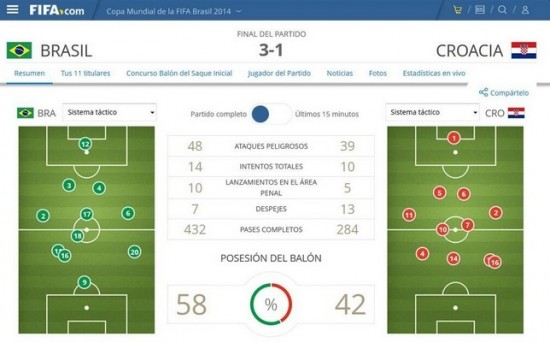
\includegraphics[scale=0.5]{img/estadistica.jpg}
    \end{figure}
\end{frame}

\begin{frame}{Aplicaciones}
    % Permite que un robot sepa de que manera tomar un objeto y usarlo como
    % herramienta de trabajo
    \begin{figure}[t]
        \centering
        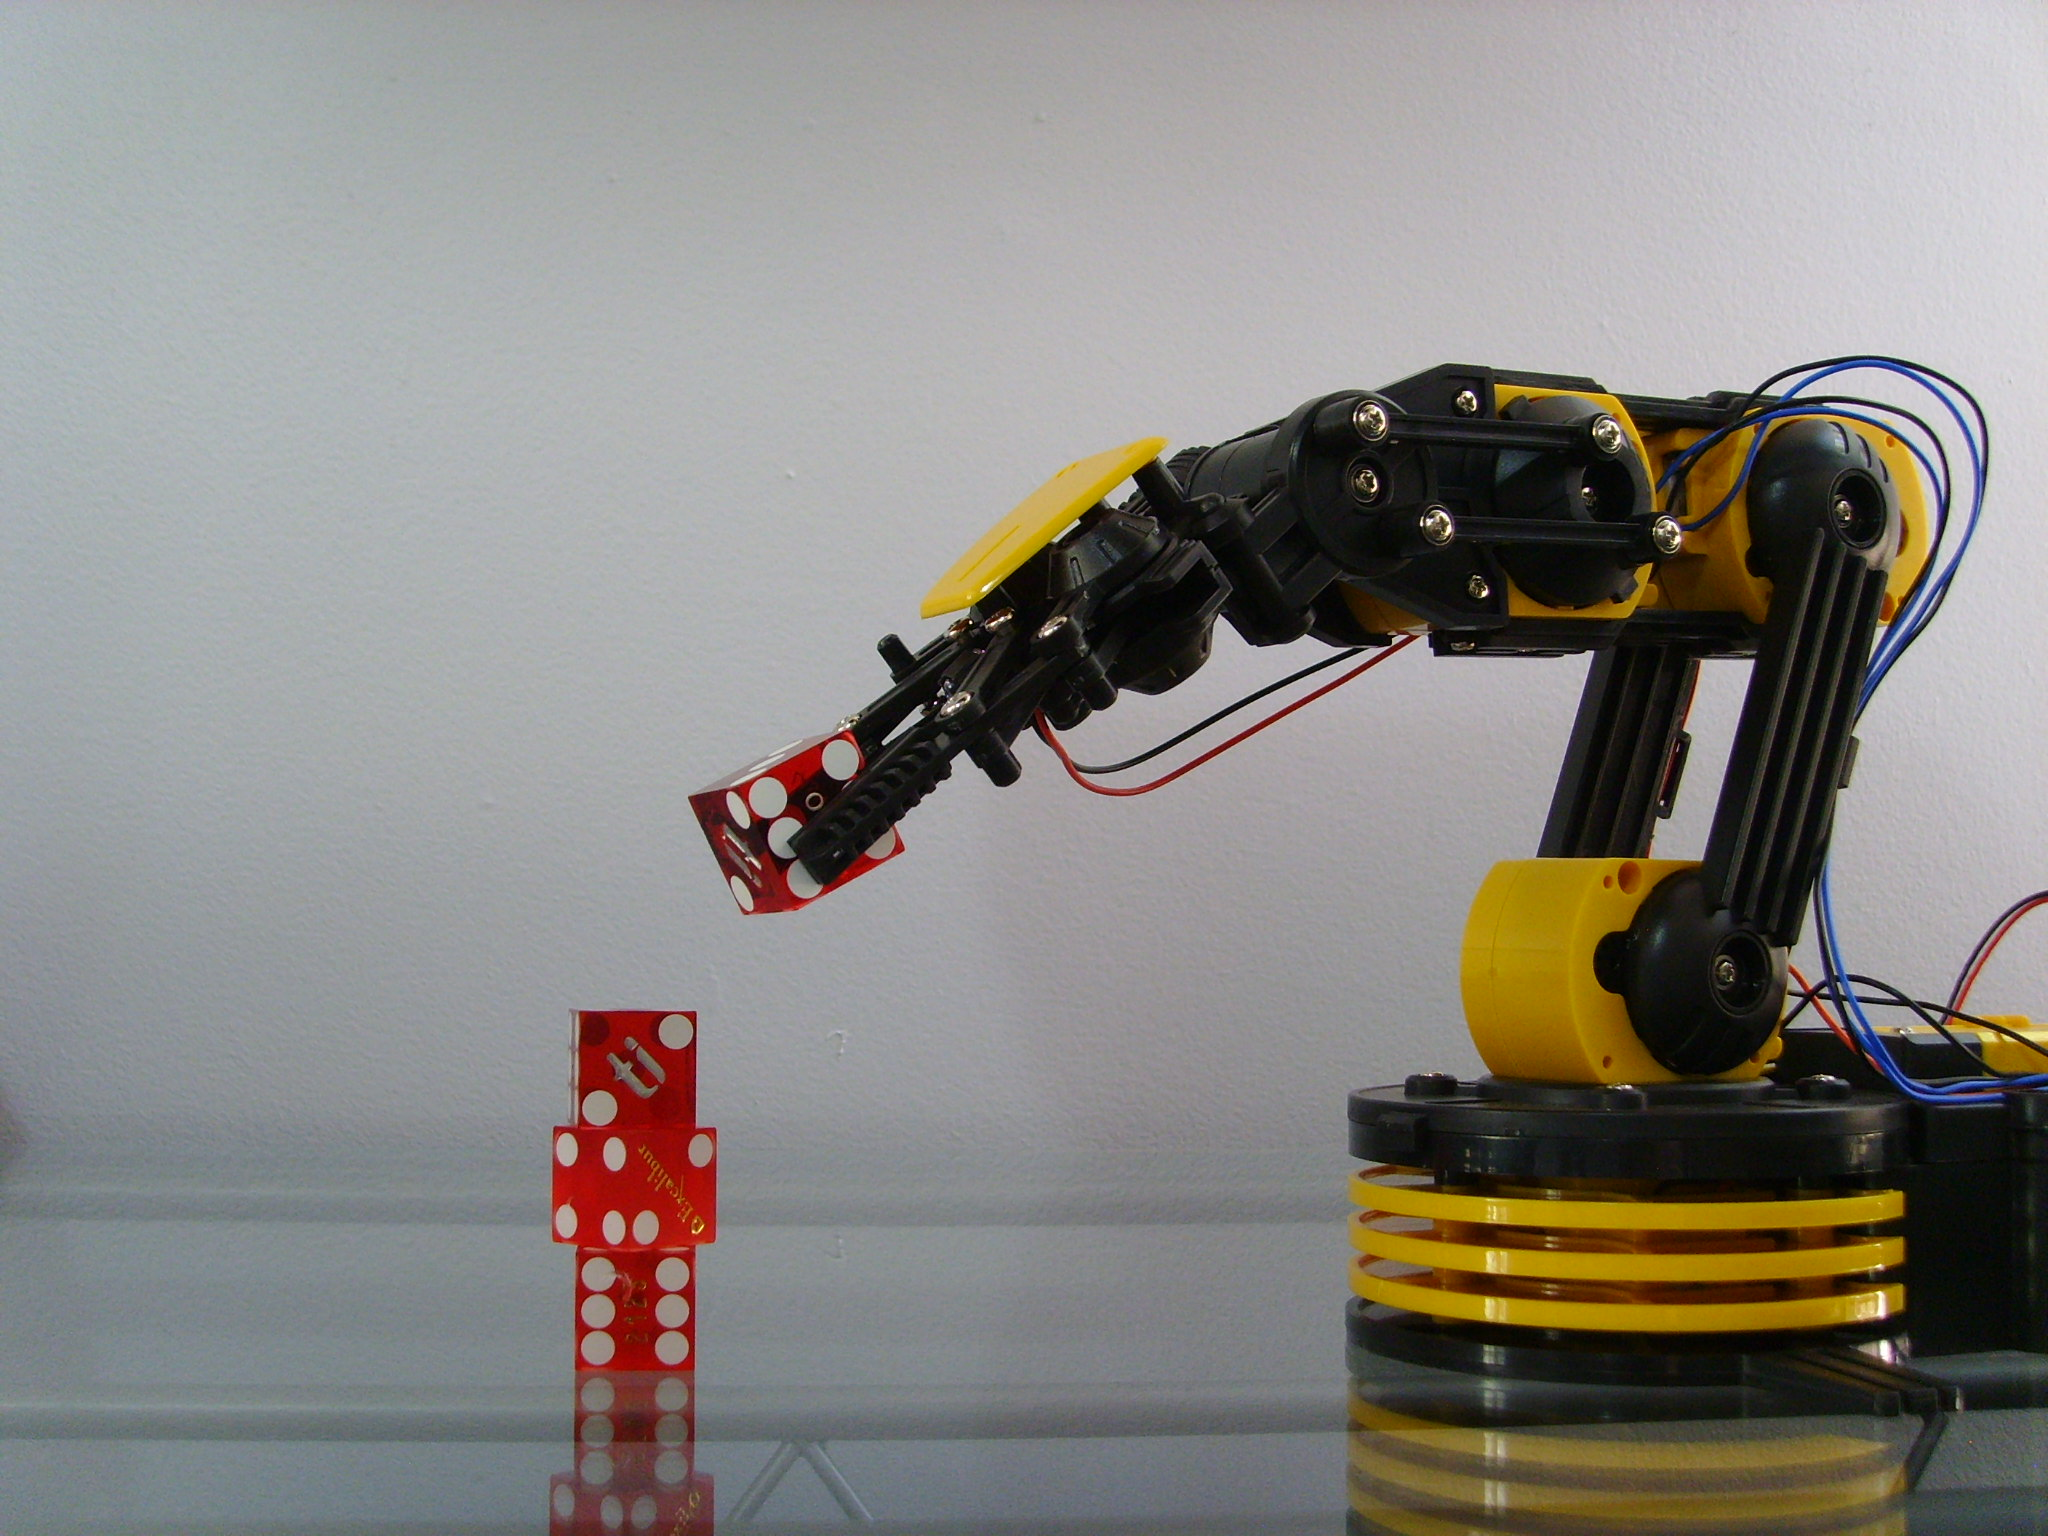
\includegraphics[scale=0.12]{img/robot.jpg}
    \end{figure}
\end{frame}

\subsection{Vamos por partes...(NO SE COMO LLAMAR A ESTO)}
\begin{frame}{Seguimiento}
    % El comportamiento esperado de un método de seguimiento es obtener para
    % cada imagen de una secuencia de imágenes o video la ubicación de un
    % objeto en algún eje de coordenadas elegido
    IMAGEN DE UN FRAME CON EL OBJETO EN UN RECUADRO Y MARCANDO LAS COORDENADAS
    DE LOS PIXELES QUE LO DESCRIBEN
\end{frame}
%--- Next Frame ---%



\begin{frame}{Objetos}
    \begin{figure}[t]
        \centering
        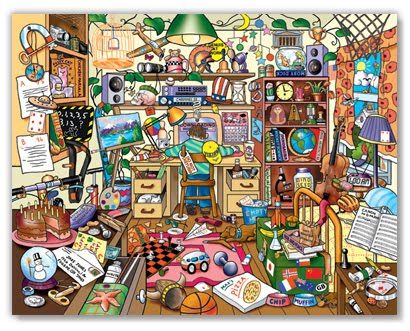
\includegraphics[scale=0.6]{img/escena_con_objetos.jpg}
    \end{figure}
\end{frame}
%--- Next Frame ---%



\begin{frame}{Secuencia de imágenes}
    % Puede ser un video, una ráfaga de imágenes tomada con una cámara de fotos
    \begin{figure}[t]
        \centering
        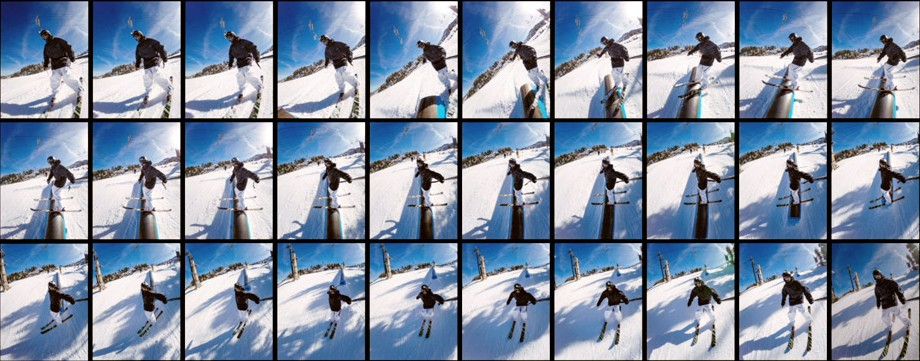
\includegraphics[scale=0.35]{img/rafaga_1.jpg}
    \end{figure}
\end{frame}
%--- Next Frame ---%



\begin{frame}{El RGB de las imágenes RGB-D}
    % Una imagen RGB-D está compuesta por dos partes. Una de ellas es una
    % imagen RGB
    % Las imágenes RGB son las más comunes y que todos conocen. Es simplemente
    % una fotografía. RGB significa Red Green Blue, que son los colores
    % primarios lumínicos (en el dominio de la luz), es decir, que el resto de los colores puede definirse
    % con una combinación de estos tres colores
    \begin{block}{}
        PEGAR UNA IMAGEN RGB CUALQUIERA
    \end{block}
\end{frame}
%--- Next Frame ---%

\begin{frame}{El D de las imágenes RGB-D}
    % Un sensor RGB-D cuenta con una cámara tipo webcam que otorga imagenes RGB,
    % un proyector infrarrojo y una cámara infrarroja. El proyector dibuja un patrón
    % conocido en la escena, que al ser infrarrojo es invisible al ojo humano.
    % Luego la cámara infrarroja captura ese patrón proyectado y utilizando algoritmos
    % de luz estructurada junto con las distancias conocidas entre la cámara y proyector
    % infrarrojo se puede obtener la profundidad para cada pixel de la escena.
    \begin{block}{}
        MOSTRAR SENSOR RGB-D, contar como funciona y mostrar con el pcl\_viewer una nube de puntos y una imagen RGB-D
    \end{block}
\end{frame}
%--- Next Frame ---%


\begin{frame}[t]{Sistema de seguimiento}
    % Un sistema de seguimiento tiene al menos 3 etapas bien definidas
    \begin{figure}[t]
        \centering
        \vspace{-13pt}
        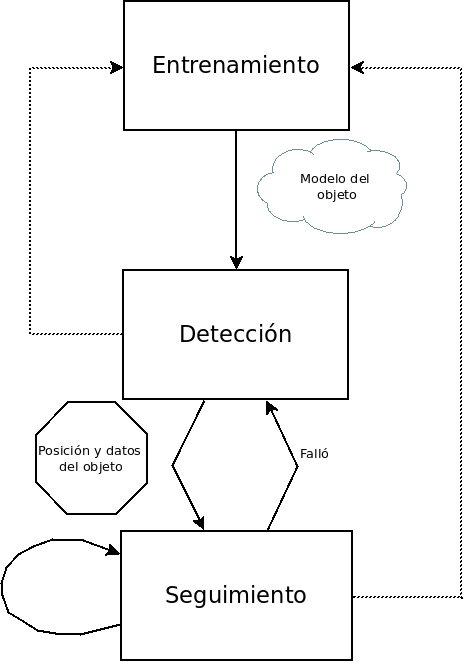
\includegraphics[scale=0.3]{img/esquema_seguimiento.png}
    \end{figure}
\end{frame}
%--- Next Frame ---%


\subsection{Objetivos}
\begin{frame}[t]{Objetivos}
    \begin{block}{Sistema RGB-D}
        Implementar, estudiar y evaluar un sistema de seguimiento RGB-D, enfocándonos especialmente en la etapa de seguimiento
    \end{block}
    \begin{block}{Análisis}
        Comparar métodos de seguimiento en RGB y en profundidad y comprender en que casos es conveniente usar uno u otro método, cuándo y de qué manera combinarlos
    \end{block}
    % TODO: preguntar por esto
    \begin{block}{Aportes???}
        Obtener resultados que puedan ser utilizados como base de comparación frente a otros sistemas de seguimiento
    \end{block}
\end{frame}
%--- Next Frame ---%



%%%%%%%%%%%%%%%%%%%%%%%%%%
%%%%%%%%%%%%%%%%%%%%%%%%%%
\section{Desarrollo}
\begin{frame}{Desarrollo}
    \begin{itemize}
        \item motivaciones, por que la separacion de los metodos, comparar metodos rgb y d
        \item explicacion de los métodos, con ejemplos en imagenes
        \item algun video de ejemplo sobre lo que se espera del sistema
    \end{itemize}

\end{frame}
%--- Next Frame ---%



%%%%%%%%%%%%%%%%%%%%%%%%%%
%%%%%%%%%%%%%%%%%%%%%%%%%%
\section{Resultados}
\begin{frame}{Resultados}
    \begin{itemize}
        \item base de datos
        \item objetos y escenas elegidos para seleccion de parametros
        \item seleccion/exploracion de parametros
        \item analisis sobre los metodos
        \item resultados por método y del sistema
        \item resultados del sistema con nuevos objetos
    \end{itemize}
\end{frame}
%--- Next Frame ---%


%%%%%%%%%%%%%%%%%%%%%%%%%%
%%%%%%%%%%%%%%%%%%%%%%%%%%
\section{Conclusiones y trabajo a futuro}
\begin{frame}{Conclusiones y trabajo a futuro}
    \begin{itemize}
        \item conclusiones
        \item mejoras a implementar
    \end{itemize}
\end{frame}
%--- Next Frame ---%


\end{document}
